% Archivo: proyecto.tex
% Archivo principal que incluye la configuración y el contenido del documento

\makeatletter
\def\input@path{{./config/}{./capitulos/}{./portada/}{./prefacios/}}
\makeatother


% !TeX root = ../proyecto.tex

% Archivo: config.tex
% Configuraciones generales, paquetes y definiciones

\documentclass[a4paper,11pt]{book}

\makeatletter
\def\input@path{{./config/}{./capitulos/}{./portada/}{./prefacios/}}
\makeatother

\usepackage{listings}
\usepackage[utf8]{inputenc}
\usepackage[spanish]{babel}
\decimalpoint
\usepackage{dcolumn}
\usepackage{fancyhdr}
\setlength{\headheight}{25.3pt}
\addtolength{\topmargin}{-7.3pt}
\usepackage{graphicx}
\usepackage{afterpage}
\usepackage[colorlinks=false, pdfborder={0 0 1}, pdfborderstyle={/S/U/W 1}]{hyperref}
\usepackage{colortbl,longtable}
\usepackage[stable]{footmisc}
\usepackage{verbatim}
\usepackage{datetime}
\usepackage{booktabs}
\usepackage{adjustbox}
\usepackage{breakurl}
\usepackage{pgfgantt} % Paquete para diagramas de Gantt
\usepackage[T1]{fontenc}
\usepackage[utf8]{inputenc}
\usepackage{lmodern}

\PassOptionsToPackage{hyphens}{url}

\usepackage[backend=biber, defernumbers=true, citestyle=numeric-comp, bibstyle=ieee, sorting=none]{biblatex}

\DeclareBibliographyCategory{cited}
\AtEveryCitekey{\addtocategory{cited}{\thefield{entrykey}}}
% Configurando BibLaTeX
\DefineBibliographyStrings{spanish}{
  url = {URL},
  andothers={et ~al\adddot}
}
\addbibresource{bibliografia/bibliografia.bib}
% Incluyo todas las referencias en la bibliografía para ver las que no se han citado
\nocite{*}

% Columnas con punto decimal español
\newcolumntype{.}{D{.}{\esperiod}{-1}}
\makeatletter
\addto\shorthandsspanish{\let\esperiod\es@period@code}
\makeatother

\addto\captionsspanish{\renewcommand{\tablename}{Tabla}}


% Información reutilizable
\newcommand{\myTitle}{Algoritmos memeticos para reducir datos de entrenamiento en modelos de aprendizaje profundo convolucionales\xspace}
\newcommand{\myDegree}{Grado en Ingeniería Informática\xspace}
\newcommand{\myName}{JOSE RUIZ LOPEZ (alumno)\xspace}
\newcommand{\myProf}{DANIEL MOLINA CABRERA (tutor)\xspace}
\newcommand{\myFaculty}{Escuela Técnica Superior de Ingenierías Informática y de Telecomunicación\xspace}
\newcommand{\myDepartment}{Departamento de Ciencias de la Computación e Inteligencia Artificial\xspace}
\newcommand{\myUni}{\protect{Universidad de Granada}\xspace}
\newcommand{\myLocation}{Granada\xspace}
\newcommand{\myTime}{\today\xspace}
\newcommand{\myVersion}{Version 0.1\xspace}


% Configuración de hyperlinks
\hypersetup{
  pdfauthor = {\myName —(ruizlopezjose@correo.ugr.es)},
  pdftitle = {\myTitle},
  pdfsubject = {Trabajo Fin de Grado},
  pdfkeywords = {Algoritmos memeticos, Imagenes, Modelos de Aprendizaje profundo convolucionales},
  pdfcreator = {LaTeX con el paquete PDFLatex y Biber},
  pdfproducer = {PDFLatex},
  breaklinks=true
}

% Definición de teoremas y otros entornos
\newtheorem{teorema}{Teorema}[chapter]
\newtheorem{ejemplo}{Ejemplo}[chapter]
\newtheorem{definicion}{Definición}[chapter]

% Configuración de listings para código
\lstset{
  frame=Ltb, framerule=0.5pt, aboveskip=0.5cm, framextopmargin=3pt,
  framexbottommargin=3pt, framexleftmargin=0.1cm, framesep=0pt, rulesep=.4pt,
  backgroundcolor=\color{gray97}, rulesepcolor=\color{black},
  stringstyle=\ttfamily, showstringspaces=false, basicstyle=\scriptsize\ttfamily,
  commentstyle=\color{gray45}, keywordstyle=\bfseries, numbers=left,
  numbersep=6pt, numberstyle=\tiny, breaklines=true
}


% Definiciones adicionales
\newcommand{\HRule}{\rule{\linewidth}{0.5mm}}

\pagestyle{fancy}
\fancyhf{}
\fancyhead[LO]{\leftmark}
\fancyhead[RE]{\rightmark}
\fancyhead[RO,LE]{\textbf{\thepage}}
\renewcommand{\chaptermark}[1]{\markboth{\textbf{#1}}{}}
\renewcommand{\sectionmark}[1]{\markright{\textbf{\thesection. #1}}}

\setlength{\headheight}{1.5\headheight}
\setlength{\parskip}{6pt}       % espacio vertical del salto de linea
\setlength{\parindent}{15pt}    % espacio de la sangría

\newcommand{\monthnamecaps}[1]{%
  \ifcase#1
  \or Enero%
  \or Febrero%
  \or Marzo%
  \or Abril%
  \or Mayo%
  \or Junio%
  \or Julio%
  \or Agosto%
  \or Septiembre%
  \or Octubre%
  \or Noviembre%
  \or Diciembre%
  \fi}

\newdateformat{mesanyo}{\monthnamecaps{\THEMONTH} de \THEYEAR}  % Importa las configuraciones desde config.tex

\begin{document}

% Portada y prefacio
% !TeX root = ../proyecto.tex

\begin{titlepage}


    \newlength{\centeroffset}
    \setlength{\centeroffset}{-0.5\oddsidemargin}
    \addtolength{\centeroffset}{0.5\evensidemargin}
    \thispagestyle{empty}

    \noindent\hspace*{\centeroffset}\begin{minipage}{\textwidth}

        \centering
        
\includegraphics[width=0.9\textwidth]{imagenes/logo_ugr.jpg}\\[1.4cm]

        \textsc{ \Large TRABAJO FIN DE GRADO\\[0.2cm]}
        \textsc{ INGENIERÍA INFORMATICA }\\[1cm]
        % Upper part of the page
        % 
        % Title
        {\Huge\bfseries Algoritmos meméticos para reducir datos de entrenamiento en modelos de aprendizaje profundo convolucionales\\
        }
        \vspace{0.2cm}
        \noindent\rule[-1ex]{\textwidth}{3pt}\\[3.5ex]
        %{\large\bfseries Subtitulo del Proyecto}
        %\end{minipage}

        \vspace{0.4cm}
        %\noindent\hspace*{\centeroffset}\begin{minipage}{\textwidth}
        %\centering

        \textbf{Autor}\\ {José Ruiz López (alumno)}\\[2.5ex]
        \textbf{Directores}\\
        {Daniel Molina Cabrera (tutor)}\\
        \vspace{0.6cm}
        
\includegraphics[width=0.3\textwidth]{imagenes/etsiit_logo.png}\\[0.1cm]
        \textsc{Escuela Técnica Superior de Ingenierías Informática y de Telecomunicación}\\
        \textsc{---}\\
        Granada, Noviembre de 2024
    \end{minipage}
    %\addtolength{\textwidth}{\centeroffset}
    %\vspace{\stretch{2}}
\end{titlepage}



% !TeX root = ../proyecto.tex

\chapter*{}
%\thispagestyle{empty}
%\cleardoublepage

%\thispagestyle{empty}


\cleardoublepage
\thispagestyle{empty}

\begin{center}
       {\large\bfseries Algoritmos meméticos para reducir datos de entrenamiento en modelos de aprendizaje profundo
              convolucionales}\\
\end{center}
\begin{center}
       José Ruiz López (alumno)\\
\end{center}

%\vspace{0.7cm}
\noindent{\textbf{Palabras clave}: Algoritmos meméticos, Imágenes, Modelos de Aprendizaje profundo convolucionales}\\

\vspace{0.7cm}
\noindent{\textbf{Resumen}}\\

Los \textbf{modelos de Aprendizaje Profundo} (Deep Learning) han supuesto un verdadero hito en la
\textbf{Inteligencia Artificial}, ya que son capaces de procesar grandes volúmenes de datos, además de reconocer
patrones sumamente complejos.
Dentro de estos, los \textbf{modelos convolucionales} se han destacado como particularmente efectivos a la hora de
identificar objetos y características en imágenes, una capacidad esencial para muchas aplicaciones modernas.
Sin embargo, a diferencia de los seres humanos, estos modelos requieren una gran cantidad de datos de
entrenamiento para cada categoría que deben aprender.
Esto implica un proceso de entrenamiento más largo y, muchas veces, la recolección de los datos necesarios puede ser
problemática, según el tipo de información que se necesite.

Además de la dificultad en la obtención de datos,  las nuevas normativas europeas en torno a la inteligencia artificial
establecen la necesidad de auditar no solo los modelos, sino también los datos
utilizados para entrenarlos, especialmente cuando se trata de aplicaciones de IA que manejan datos sensibles.
Estas auditorías, por su propia naturaleza, se volverán más complejas conforme aumente el tamaño del conjunto de
entrenamiento.
Por lo tanto, se vuelve completamente necesario desarrollar estrategias que permitan
\textbf{reducir el tamaño de los conjuntos de datos de entrenamiento} intentado comprometer la calidad del modelo lo mínimo posible.

En este trabajo, proponemos el uso de \textbf{algoritmos meméticos} para establecer un proceso de reducción del conjunto de
\textbf{entrenamiento}, lo que se conoce como \textbf{selección de instancias}.
La idea es seleccionar un conjunto reducido de imágenes representativas que, junto con las técnicas de aumento de
datos, sean suficientes para entrenar modelos convolucionales de manera óptima.
De este modo, se podría reducir significativamente el tamaño del conjunto de entrenamiento, manteniendo la calidad
del aprendizaje y, a su vez, facilitando tanto el proceso de auditoría como la eficiencia computacional del sistema.


\cleardoublepage


\thispagestyle{empty}


\begin{center}
       {\large\bfseries Memetic Algorithms for Reducing Training Data in Convolutional Deep Learning Models}\\
\end{center}
\begin{center}
       José, Ruiz López (student)\\
\end{center}

%\vspace{0.7cm}
\noindent{\textbf{Keywords}: Memetic Algorithms, Images, Convolutional Deep Learning Models}\\

\vspace{0.7cm}
\noindent{\textbf{Abstract}}\\

\textbf{Deep Learning models} have marked a true milestone in the field of \textbf{Artificial Intelligence}, as they are capable of 
processing large volumes of data and recognizing highly complex patterns.
Among these, \textbf{convolutional models} have stood out as particularly effective in identifying objects and
features in images, an essential capability for many modern applications.
However, unlike humans, these models require a large amount of training data for each category they need to learn.
This implies a longer training process, and in many cases, collecting the necessary data can be problematic depending
on the type of information required.

In addition to the difficulty of obtaining data, new European regulations on artificial intelligence establish the need to 
audit not only the models but also the data used to train them, especially in AI applications that handle sensitive data.
These audits, by their very nature, will become increasingly complex as the size of the training set grows.
Therefore, it becomes essential to develop strategies that allow for \textbf{reducing the size of training datasets}, 
while minimizing any compromise in model quality.

In this work, we propose the use of \textbf{memetic algorithms} to implement a \textbf{training data reduction process}, 
also known as \textbf{instance selection}.
The idea is to select a small set of representative images that, along with data augmentation techniques, 
are sufficient to optimally train convolutional models.
In this way, it would be possible to significantly reduce the size of the training set while maintaining learning quality and, 
at the same time, facilitating both the auditing process and the system's computational efficiency.

\chapter*{}
\thispagestyle{empty}

\noindent\rule[-1ex]{\textwidth}{2pt}\\[4.5ex]

Yo, \textbf{José Ruiz López}, alumno de la titulación INGENIERÍA INFORMÁTICA de la \textbf{Escuela Técnica Superior
       de Ingenierías Informática y de Telecomunicación de la Universidad de Granada}, con DNI \textbf{77964364E}, autorizo la
ubicación de la siguiente copia de mi Trabajo Fin de Grado en la biblioteca del centro para que pueda ser
consultada por las personas que lo deseen.

\vspace{6cm}

\noindent Fdo: José Ruiz López

\vspace{2cm}

\begin{flushright}
       Granada a \today.
\end{flushright}


\chapter*{}
\thispagestyle{empty}

\noindent\rule[-1ex]{\textwidth}{2pt}\\[4.5ex]

D. \textbf{Daniel Molina Cabrera (tutor}, Profesor del Departamento Ciencias de la Computación e Inteligencia
Artificial de la Universidad de Granada.

\vspace{0.5cm}

\textbf{Informan:}

\vspace{0.5cm}

Que el presente trabajo, titulado \textit{\textbf{Algoritmos meméticos para reducir datos de entrenamiento en modelos de aprendizaje profundo convolucionales}},
ha sido realizado bajo su supervisión por \textbf{José Ruiz López (alumno)}, y autorizamos la defensa de dicho trabajo  ante el tribunal que corresponda.

\vspace{0.5cm}

Y para que conste, expiden y firman el presente informe en Granada a \today.

\vspace{1cm}

\textbf{Los directores:}

\vspace{5cm}

\noindent \textbf{Daniel Molina Cabrera (tutor)}

\chapter*{Agradecimientos}
\thispagestyle{empty}

\vspace{1cm}


Quiero expresar mi más sincero agradecimiento a todas las personas que han hecho posible la realización de este Trabajo de Fin de Grado.

En primer lugar, me gustaría agradecer al profesor Daniel Molina Cabrera, mi tutor, por su valiosa guía, por su apoyo continuo durante 
todo el proceso y por brindarme acceso a los recursos necesarios para llevar a cabo esta investigación.
Su experiencia y disponibilidad han sido fundamentales para que este proyecto pudiera desarrollarse de forma rigurosa y enriquecedora.

También quiero destacar lo desafiante que ha sido compaginar este trabajo académico con mis responsabilidades laborales.
Ha requerido un esfuerzo constante y una gran capacidad de organización, pero también me ha permitido valorar aún más el proceso y el aprendizaje adquirido.

Agradezco de corazón a mis padres y amigos por su comprensión, paciencia y apoyo emocional durante los momentos más exigentes del camino.
Y, sobre todo, a mi pareja, sin ella no habría sido posible superar el reto que supone realizar un trabajo como este. 
Su apoyo incondicional, su confianza en mí y la calma que me ha transmitido en los momentos más difíciles han sido clave para llegar hasta el final.

Asimismo, extiendo mi gratitud a todas las personas y compañeros que, directa o indirectamente, han contribuido con sus comentarios, sugerencias y tiempo.
Gracias a ellos, este trabajo ha podido alcanzar una mayor profundidad y claridad.

Por último, quiero agradecer a todas aquellas comunidades de código abierto y herramientas libres que han permitido que este proyecto se 
desarrollara sin barreras tecnológicas, facilitando el aprendizaje y la innovación.


% Índices
\frontmatter
\tableofcontents
%\listoffigures
%\listoftables

% Cuerpo del documento
\mainmatter
% !TeX root = ../proyecto.tex

\chapter{Introducción}\label{ch:introduccion}

%Contexto: Breve introducción al tema y su relevancia.
En la actualidad, vivimos en una era marcada por una constante y acelerada generación de datos.
Este fenómeno ha incrementado la necesidad de desarrollar métodos eficaces para el procesamiento y análisis de grandes
volúmenes de información.
En este contexto, los \textbf{modelos de aprendizaje profundo}, y en particular las
\textbf{redes neuronales convolucionales} (CNN), han demostrado un notable rendimiento en tareas como la
\textbf{clasificación de imágenes}, el \textbf{reconocimiento de patrones} y diversas aplicaciones de alta complejidad.
No obstante, el entrenamiento de estos modelos suele requerir volúmenes elevados de datos, lo que plantea desafíos
significativos tanto en términos de \textbf{tiempo} como de \textbf{costes} asociados a su obtención.



Conforme los sistemas de inteligencia artificial evolucionan hacia estructuras más sofisticadas y precisas, la
disponibilidad de conjuntos de datos amplios y adecuados se vuelve un requisito cada vez más crucial.
Sin embargo, la recopilación, almacenamiento y tratamiento de estos datos suponen obstáculos importantes, especialmente
para aquellas instituciones u organizaciones que cuentan con recursos limitados.
Esta situación pone de relieve la necesidad de investigar estrategias innovadoras que permitan
\textbf{reducir y optimizar los conjuntos de datos} sin comprometer el rendimiento de los modelos entrenados.


En consecuencia, surge la necesidad de \textbf{reducir los conjuntos de datos de entrenamiento}
para mejorar la \textbf{eficiencia} en el desarrollo de modelos de aprendizaje profundo.
Aunque las redes neuronales convolucionales han demostrado un rendimiento notable en diversas tareas, su implementación
conlleva \textbf{altos costes computacionales} y una gran demanda de datos, lo que  supone un obstáculo importante en muchos escenarios,
especialmente aquellos con recursos limitados.
Una estrategia prometedora consiste en entrenar estos modelos utilizando únicamente una fracción de los datos
disponibles, seleccionados de manera óptima.
Esta aproximación permitiría disminuir significativamente el consumo de recursos sin comprometer la precisión del
modelo, lo que supondría un avance importante para la \textbf{inteligencia artificial}, en particular en aplicaciones
donde existen \textbf{restricciones de recursos}.


En este contexto, la selección inteligente de subconjuntos representativos constituye una estrategia eficaz para reducir tanto
los tiempos de entrenamiento como el uso de recursos, sin afectar negativamente el rendimiento.
Es precisamente en este punto donde las \textbf{metaheurísticas} adquieren un papel relevante.
Estas técnicas de optimización están diseñadas para abordar problemas complejos en los que los métodos tradicionales
resultan ineficaces, gracias a sus \textbf{estrategias de búsqueda} y \textbf{exploración del espacio de soluciones}.
Al combinar diversas heurísticas, permiten encontrar soluciones aproximadas en tiempos razonables, lo que las convierte
en una herramienta especialmente útil cuando la obtención de una solución exacta resulta inviable desde el punto de
vista computacional.


Gracias a estas características, las metaheurísticas se posicionan como una alternativa sólida
para mejorar la eficiencia y accesibilidad del aprendizaje profundo, incluso en contextos con recursos limitados.
Esto es especialmente relevante para avanzar hacia una inteligencia artificial más abierta, \textbf{democrática} y aplicable
en una mayor variedad de escenarios.


En este contexto, el presente Trabajo de Fin de Grado tiene como objetivo aplicar técnicas metaheurísticas para realizar una selección
inteligente de ejemplos, con el fin de reducir el tamaño de los conjuntos de entrenamiento sin que ello afecte
significativamente a los resultados obtenidos.
La investigación aspira a contribuir al desarrollo de modelos más \textbf{eficientes}, accesibles y económicamente
sostenibles, fomentando así un futuro en el que la inteligencia artificial sea más \textbf{inclusiva} y
\textbf{sostenible}.


%Objetivos: Especifica qué pretendes lograr con tu TFG.
El objetivo principal de este TFG es investigar la aplicación de \textbf{metaheurísticas} para la
\textbf{reducción de conjuntos de datos de entrenamiento} en modelos de \textbf{aprendizaje profundo convolucionales}.
Este estudio permitirá evaluar el impacto de dichos algoritmos en la \textbf{eficiencia computacional} y en el
\textbf{rendimiento de los modelos}.
Para lograr estos objetivos, se desarrollarán y compararán distintas técnicas de selección de instancias aplicadas
sobre modelos convolucionales, incluyendo enfoques aleatorios, de búsqueda local, genéticos y meméticos.


Para cumplir con este objetivo general, se plantean los siguientes \textbf{objetivos específicos}:

\begin{itemize}
      \item \textbf{Estudiar} la conveniencia del uso de metaheurísticas para la reducción de conjuntos de imágenes
            en modelos de aprendizaje profundo.
      \item \textbf{Desarrollar} y \textbf{mejorar} algoritmos metaheurísticos orientados a la selección de ejemplos representativos,
            con el objetivo de optimizar el entrenamiento de modelos convolucionales sin comprometer su rendimiento.
      \item \textbf{Evaluar} el impacto de la reducción de datos en el rendimiento de los modelos, comparando aspectos clave
            como la precisión, eficacia y el tiempo de entrenamiento, en modelos entrenados con conjuntos de datos completos frente a conjuntos reducidos.
      \item \textbf{Comparar} el rendimiento de metaheurísticas con porcentajes de selección fijos frente a aquellos que
            permiten una selección flexible del número de ejemplos, analizando sus ventajas y limitaciones.
\end{itemize}

A través de este estudio, se busca no solo mejorar el rendimiento y la eficiencia de los modelos convolucionales,
sino también fomentar el desarrollo de soluciones más \textbf{sostenibles y accesibles} en el ámbito de la inteligencia artificial,
mediante la incorporación de estrategias metaheurísticas como \textbf{propuestas innovadoras} para la reducción de datos de entrenamiento.

Este trabajo se enmarca en el Proyecto ``Inteligencia Artificial Ética, Responsable y de Propósito General: Aplicaciones En Escenarios De Riesgo.'' (IAFER) Exp.:TSI-100927-2023-1.

% !TeX root = ../proyecto.tex

\chapter{Metodología y Presupuesto}\label{ch:metodologia-y-presupuesto}
\section{Metodología}\label{sec:metodologia}
Para organizar el desarrollo del proyecto se optó por una metodología inspirada en el marco ágil
\textbf{Scrum}~\cite{ScrumGuide}, ampliamente utilizado en entornos donde se requiere adaptación constante y
entregas progresivas.
Dado que el desarrollo del trabajo se ajustaba progresivamente según los resultados obtenidos en cada fase,
este enfoque demostró ser adecuado para mantener una estructura flexible y favorecer un avance iterativo

\subsection{Enfoque Ágil Basado en Scrum}\label{subsec:enfoque-agil-basado-en-scrum}
El proyecto se dividió en ciclos de trabajo breves (\textbf{sprints}), generalmente de dos semanas.
Cada sprint comenzaba con una planificación en la que se establecían objetivos concretos y finalizaba con una revisión
para evaluar el progreso y hacer ajustes si era necesario.
Esta dinámica permitió mantener un ritmo constante, al tiempo que se dejaba margen para adaptarse a posibles
imprevistos o nuevas ideas surgidas durante el desarrollo.

\subsection{Organización de Tareas}\label{subsec:organizacion-de-tareas}
Para la organización y seguimiento de tareas se empleó una herramienta digital de apoyo (Notion~\cite{NotionGestionTareas}),
que facilitó la planificación personal y visualización de actividades pendientes.


Este tipo de plataformas contribuyen a mejorar la organización y la colaboración en proyectos complejos,
tal como se ha demostrado en entornos profesionales mediante el uso de tecnologías de la información orientadas a la gestión colaborativa~\cite{EnhancingCollaborationProjectbased}.


Esta plataforma facilitó la visualización de las actividades pendientes y cumplidas, lo que ayudó a no perder de vista
los plazos y prioridades de cada fase.


En paralelo, se empleó \textbf{Git}~\cite{chaconProGit2014} para el control de versiones del código, lo que resultó
fundamental para mantener un seguimiento detallado de los cambios realizados en cada etapa del proyecto.
También se utilizó \textbf{GitHub} como repositorio central, facilitando así la colaboración con el tutor y permitiendo
una trazabilidad clara de todas las modificaciones.
El código fuente completo y los recursos del proyecto están disponibles en el repositorio: \url{https://github.com/JoseRuizLopez/TFG}.


\subsection{Ciclos de Trabajo}\label{subsec:ciclos-de-trabajo}
Los sprints se estructuraron en varias fases repetidas en cada iteración:

\begin{itemize}
    \item \textbf{Planificación}: En esta etapa se definían los objetivos del sprint, basándose en lo ya realizado y en
          las tareas pendientes más prioritarias.
          El análisis del \textbf{backlog} permitía seleccionar actividades realistas que se pudieran completar en el plazo
          previsto.

    \item \textbf{Desarrollo e implementación}: Se ejecutaban las tareas previstas, como la programación de nuevos
          módulos, mejoras en algoritmos o la integración de componentes.
          El enfoque fue incremental, es decir, se añadían funcionalidades poco a poco, asegurando que cada avance se pudiera
          probar por separado.

    \item \textbf{Pruebas y ajustes}: Una vez desarrolladas las funcionalidades, se realizaban pruebas (unitarias, de
          integración o empíricas) para validar el funcionamiento del sistema y ajustar los parámetros si fuese necesario.
          A veces, los resultados de esta fase daban lugar a nuevas tareas que se añadían al backlog.

    \item \textbf{Revisión y análisis de resultados}: Al finalizar el sprint, se revisaban los objetivos cumplidos, se
          analizaban los resultados obtenidos y se valoraba la necesidad de replantear enfoques.
          Esta revisión también ayudaba a identificar puntos de mejora y reforzar los que ya funcionaban bien.

    \item \textbf{Documentación}: Durante todo el proceso se fue registrando la evolución del proyecto, desde los
          cambios en el código hasta los resultados de las pruebas.
          Este esfuerzo permitió tener una memoria bien estructurada, facilitar la reproducción de experimentos y justificar cada
          decisión tomada.
\end{itemize}


\newpage
\subsection{Seguimiento del Progreso}\label{subsec:seguimiento-del-progreso}

\begin{figure}[htp]
    \definecolor{sprint_color1}{RGB}{51,102,254} % Azul oscuro para Sprint 1
    \definecolor{sprint_color2}{RGB}{38, 173, 70} % Verde oscuro para Sprint 2
    \definecolor{fase_color1}{RGB}{153,204,254} % Azul claro para Fase 1
    \definecolor{fase_color2}{RGB}{138, 222, 158} % Verde claro más oscuro para Fase 2
    \renewcommand\sfdefault{phv}
    \renewcommand\mddefault{mc}
    \renewcommand\bfdefault{bc}
    \sffamily
    \noindent
    \resizebox{\textwidth}{!}{
        \begin{ganttchart}[
                group label node/.append style={anchor=east}, % Alinea grupo a la derecha
                bar label node/.append style={anchor=east}, % Alinea fases a la derecha
                group left shift=0,
                canvas/.append style={fill=none, draw=black!5, line width=.75pt},
                hgrid style/.style={draw=black!5, line width=.75pt},
                vgrid={*1{draw=black!5, line width=.75pt}},
                today label font=\small\bfseries,
                title/.style={draw=none, fill=none},
                title label font=\bfseries\footnotesize,
                title label node/.append style={align=center}, % Centrado horizontal
                include title in canvas=false,
                bar/.append style={draw=none}, % Sin borde en las barras
                bar incomplete/.append style={fill=barblue},
                group right shift=0,
                group height=.5,
                group peaks tip position=0,
                group progress label font=\bfseries\small,
                link/.style={-latex, line width=1.5pt, linkred},
                link label font=\scriptsize\bfseries,
                link label node/.append style={below left=-2pt and 0pt},
                x unit=0.4cm,
                y unit title=0.6cm, % Controla la altura de la fila del título
            ]{1}{27}

            % Omitimos el título DAYS en el mecanismo estándar y dejamos solo los números
            \gantttitle{1}{1} \gantttitle{2}{1} \gantttitle{3}{1} \gantttitle{4}{1} \gantttitle{5}{1}
            \gantttitle{6}{1} \gantttitle{7}{1} \gantttitle{8}{1} \gantttitle{9}{1} \gantttitle{10}{1}
            \gantttitle{11}{1} \gantttitle{12}{1} \gantttitle{13}{1} \gantttitle{14}{1} \gantttitle{15}{1}
            \gantttitle{16}{1} \gantttitle{17}{1} \gantttitle{18}{1} \gantttitle{19}{1} \gantttitle{20}{1}
            \gantttitle{21}{1} \gantttitle{22}{1} \gantttitle{23}{1} \gantttitle{24}{1} \gantttitle{25}{1}
            \gantttitle{26}{1} \gantttitle{27}{1} \gantttitle{28}{1}
            \\ % Salto de línea después de los títulos

            % Sprint 1 alineado a la derecha - con color personalizado
            \ganttgroup[name=sprint1, group/.append style={fill=sprint_color1}]{Sprint 1}{1}{14} \\
            \ganttbar[name=s1fase1, bar/.append style={fill=fase_color1}]
            {Planificación del sprint \textbf{| Fase 1}}{1}{1} \\
            \ganttbar[name=s1fase2, bar/.append style={fill=fase_color1}]
            {Desarrollo e implementación de algoritmos \textbf{| Fase 2}}{2}{4} \\
            \ganttbar[name=s1fase3, bar/.append style={fill=fase_color1}]
            {Pruebas y ajustes \textbf{| Fase 3}}{5}{10} \\
            \ganttbar[name=s1fase4, bar/.append style={fill=fase_color1}]
            {Revisión y análisis de resultados \textbf{| Fase 4}}{11}{12} \\
            \ganttbar[name=s1fase5, bar/.append style={fill=fase_color1}]
            {Documentación de los algoritmos y resultados \textbf{| Fase 5}}{13}{14} \\[grid]

            % Sprint 2 alineado a la derecha - con color personalizado
            \ganttgroup[name=sprint2, group/.append style={fill=sprint_color2}]{Sprint 2}{15}{28} \\
            \ganttbar[name=s2fase1, bar/.append style={fill=fase_color2}]
            {Planificación del sprint\textbf{| Fase 1}}{15}{15} \\
            \ganttbar[name=s2fase2, bar/.append style={fill=fase_color2}]
            {Desarrollo e implementación de algoritmos \textbf{| Fase 2}}{16}{18} \\
            \ganttbar[name=s2fase3, bar/.append style={fill=fase_color2}]
            {Pruebas y ajustes \textbf{| Fase 3}}{19}{24} \\
            \ganttbar[name=s2fase4, bar/.append style={fill=fase_color2}]
            {Revisión y análisis de resultados \textbf{| Fase 4}}{25}{26} \\
            \ganttbar[name=s2fase5, bar/.append style={fill=fase_color2}]
            {Documentación de los algoritmos y resultados \textbf{| Fase 5}}{27}{28}
        \end{ganttchart}
    }
    \caption{
        Diagrama de Gantt que muestra la planificación de dos sprints del proyecto, con sus respectivas fases: planificación,
        desarrollo, pruebas, revisión y documentación. Este esquema representa la estructura iterativa adoptada a lo largo del desarrollo
    }\label{fig:gantt-diagram}
\end{figure}

Para tener una visión clara del avance del proyecto, se elaboró un \textbf{diagrama de Gantt}~[\ref{fig:gantt-diagram}]
que recogía dos sprints como ejemplo del proceso general.
En él se reflejan las distintas fases mencionadas, así como la duración aproximada de cada una.
Aunque se realizaron más sprints a lo largo del trabajo, este diagrama sirve como muestra del esquema de planificación
utilizado.

\subsection{Ajuste de los Tiempos}\label{subsec:ajuste-de-los-tiempos}
Durante el desarrollo surgieron algunos retrasos que obligaron a reajustar los tiempos previstos para los sprints.
Gracias a la flexibilidad que permite \textbf{Scrum} y al uso de herramientas como \textbf{Git},
permitió reorganizar prioridades y redistribuir tareas sin comprometer los objetivos del proyecto sin comprometer la calidad del trabajo.

\section{Presupuesto}\label{sec:presupuesto}
El presupuesto estimado incluye tanto el tiempo dedicado al proyecto (mano de obra) como los recursos computacionales y
otros gastos relacionados.
Aunque muchos recursos utilizados son gratuitos o de bajo coste, se ha realizado una estimación considerando el valor
del tiempo invertido y el uso de recursos computacionales.

\subsection{Mano de obra}\label{subsec:mano-de-obra}
El proyecto ha requerido un esfuerzo considerable distribuido entre tareas de análisis, desarrollo e implementación técnica,
así como documentación y validación experimental.
En total, se estima que se han dedicado aproximadamente \textbf{400 horas} al trabajo, repartidas de forma flexible a lo largo del calendario del TFG.

La estimación del coste de la mano de obra se ha calculado a partir de una tarifa de \textbf{20 euros} por hora,
en línea con valores orientativos para trabajos técnicos similares~\cite{SalarioParaData}.

A continuación se detallan las tareas principales:
\begin{itemize}
    \item \textbf{Planificación inicial y diseño del proyecto}: Establecimiento de objetivos, enfoque metodológico y cronograma.
    \item \textbf{Repaso bibliográfico}: Revisión de trabajos previos relacionados con algoritmos meméticos y reducción de datos en aprendizaje profundo.
    \item \textbf{Comprensión del problema y formulación}: Definición precisa del problema y formalización de los objetivos computacionales.
    \item \textbf{Selección de datasets y preprocesado}: Búsqueda, limpieza y organización de los conjuntos de datos utilizados.
    \item \textbf{Implementación inicial de algoritmos}: Desarrollo de versiones base de los algoritmos genético, memético y de búsqueda local.
    \item \textbf{Desarrollo de versiones mejoradas}: Ajustes iterativos, experimentación con nuevas variantes y mecanismos de exploración.
    \item \textbf{Evaluación experimental y análisis de resultados}: Ejecución masiva de pruebas, análisis comparativo y visualización de métricas.
    \item \textbf{Generación de gráficos}: Creación de boxplots, barplots y figuras de evolución del fitness.
    \item \textbf{Escritura de la memoria del TFG}: Redacción estructurada del documento final, incluyendo capítulos técnicos, resultados y conclusiones.
    \item \textbf{Revisión y corrección}: Mejora del contenido tras la retroalimentación del tutor, ajuste de redacción, formato y bibliografía.
\end{itemize}


\begin{table}[htp]
    \centering
    \begin{adjustbox}{width=\linewidth}
        \begin{tabular}{|l|r|r|r|}
            \hline
            \textbf{Tarea realizada}                         & \textbf{Horas dedicadas} & \textbf{Coste por hora (€)} & \textbf{Coste total (€)} \\ \hline
            Planificación inicial y diseño del proyecto      & 20                       & 20                          & 400                      \\
            Repaso bibliográfico                             & 30                       & 20                          & 600                      \\
            Comprensión del problema y formulación           & 25                       & 20                          & 500                      \\
            Selección de datasets y preprocesado inicial     & 20                       & 20                          & 400                      \\
            Implementación inicial de algoritmos             & 40                       & 20                          & 800                      \\
            Desarrollo de propuestas y versiones mejoradas   & 50                       & 20                          & 1.000                    \\
            Evaluación experimental y análisis de resultados & 60                       & 20                          & 1.200                    \\
            Generación de gráficos                           & 30                       & 20                          & 600                      \\
            Escritura de la memoria del TFG                  & 80                       & 20                          & 1.600                    \\
            Revisión y corrección final del documento        & 45                       & 20                          & 900                      \\ \hline
            \textbf{Total}                                   & \textbf{400 horas}       &                             & \textbf{8.000 €}         \\ \hline
        \end{tabular}
    \end{adjustbox}
    \caption{Estimación detallada del coste de la mano de obra distribuido por tareas del proyecto.}
    \label{tab:mano-de-obra}
\end{table}


A modo de resumen, en la Tabla~\ref{tab:mano-de-obra} se presenta una distribución detallada de las horas dedicadas a cada una de estas tareas,
junto con el coste estimado asociado.
Esta descomposición permite visualizar de forma clara cómo se ha estructurado el esfuerzo invertido, diferenciando tareas de investigación, desarrollo técnico y documentación.
El resultado total asciende a 8.000 €, lo que proporciona una visión aproximada del valor económico del trabajo llevado a cabo.

\subsection{Recursos computacionales}\label{subsec:recursos-computacionales}
El proyecto ha requerido el uso de recursos computacionales para entrenar los modelos de aprendizaje profundo,
especialmente para evaluar la eficacia de los algoritmos en la reducción de datos.


El tutor \textbf{Daniel Molina Cabrera} me puso en disposición el acceso a un servidor de investigación con
disponibilidad de GPU, de manera que no ha supuesto ningún coste.


Aunque el acceso al servidor de investigación con GPU no implicó coste real,
se ha realizado una estimación hipotética utilizando precios de \textbf{Google Cloud}~\cite{OverviewGoogleCloud}
usando un \textbf{Compute Engine}~\cite{WhatCloudRun} en Bélgica para valorar el uso de recursos.


Los componentes equivalentes del servidor en Compute Engine serían:
\begin{itemize}
    \item Un \textbf{Intel Xeon E-2226G} equivaldría a un \textbf{c2-standard-8}, cuyo coste es de 0.43 EUR/h.
    \item Un \textbf{NVIDIA TITAN Xp} equivaldría a una \textbf{NVIDIA K80 1 GPU}, GDDR5 de 12 GB cuyo coste es de 0.42
          EUR/h.
\end{itemize}

De modo que los gastos estimados serían:
\begin{table}[htp]
    \centering
    \begin{adjustbox}{width=\linewidth}
        \begin{tabular}{|l|r|r|r|}
            \hline
            \textbf{Recurso}       & \textbf{Horas utilizadas} & \textbf{Coste por hora (€)} &
            \textbf{Coste total (€)}                                                                        \\ \hline
            CPU (c2-standard-8)    & 600                       & 0.43                        & 258          \\
            GPU (NVIDIA K80 1 GPU) & 600                       & 0.42                        & 252          \\ \hline
            \textbf{Total}         & \textbf{600}              & \textbf{0.85}               & \textbf{510} \\ \hline
        \end{tabular}
    \end{adjustbox}
    \caption{Simulación del coste de recursos computacionales equivalentes en Google Cloud.}
    \label{tab:recursos-computacionales}
\end{table}


\subsection{Software y licencias}\label{subsec:software-y-licencias}
Para este proyecto, todas las herramientas de desarrollo utilizadas han sido de \textbf{código abierto},
por lo que no se han incurrido en costes de licencias.

\subsection{Gastos indirectos}\label{subsec:gastos-indirectos}
Aunque muchos de los recursos utilizados durante el desarrollo del proyecto han sido gratuitos o provistos por el entorno universitario,
se ha considerado el coste indirecto asociado al uso continuado del equipo personal.

En concreto, se estima el coste proporcional derivado del uso de un ordenador portátil \textbf{Lenovo Ideapad 530S-14KB},
empleado intensivamente durante todo el curso académico para la programación, análisis y documentación del TFG.
El cálculo se ha realizado prorrateando su valor de adquisición estimado (aproximadamente 900 €) a lo largo de una vida útil de 5 años,
lo que da lugar a un coste anual aproximado de 180 €.

\begin{table}[htp]
    \centering
    \begin{tabular}{|l|r|}
        \hline
        \textbf{Concepto}                      & \textbf{Coste estimado (€)} \\ \hline
        Uso del portátil (Lenovo Ideapad 530S) & 180                         \\ \hline
    \end{tabular}
    \caption{Estimación de gastos indirectos asociados al desarrollo del proyecto.}
    \label{tab:gastos-indirectos}
\end{table}


\subsection{Presupuesto total}\label{subsec:presupuesto-total}
Sumando los costes de mano de obra, los recursos computacionales y otros gastos, el presupuesto total estimado es el
siguiente:

\begin{table}[htp]
    \centering
    \begin{tabular}{|l|c|}
        \hline
        \textbf{Concepto}        & \textbf{Coste (€)} \\ \hline
        Mano de obra             & 8.000              \\
        Recursos computacionales & 510                \\
        Gastos indirectos        & 180                \\ \hline
        \textbf{Total}           & \textbf{8.690 €}   \\ \hline
    \end{tabular}
    \caption{Resumen del presupuesto total estimado, incluyendo mano de obra, recursos y gastos indirectos.}
    \label{tab:presupuesto-total}
\end{table}

En conjunto, la planificación metodológica y la estimación de recursos permitieron garantizar el avance
ordenado del proyecto y anticipar su viabilidad técnica y económica.
\chapter{Fundamentos de Aprendizaje Profundo}\label{ch:fundamentos-de-aprendizaje-profundo}
%Fundamentos de Aprendizaje Profundo: Explica los conceptos básicos, incluyendo redes neuronales convolucionales.
\section{Definición de Aprendizaje Profundo}\label{sec:definicion-de-aprendizaje-profundo}
El \textbf{aprendizaje profundo} (Deep Learning) es una subcategoría del aprendizaje automático que se basa
en el uso de \textbf{redes neuronales artificiales} con muchas capas (de ahí el término ``profundo''.
Estas redes están diseñadas para imitar el funcionamiento del cerebro humano, lo que les permite aprender
representaciones complejas de los datos de manera jerárquica. \\[2pt]

La principal diferencia entre el \textbf{aprendizaje automático tradicional} y el aprendizaje profundo es la manera en
que se manejan las características de los datos:
\begin{itemize}
    \item En los enfoques tradicionales, el ingeniero o científico de datos debe extraer manualmente las
características más importantes para entrenar al modelo (por ejemplo, bordes, formas, texturas en imágenes).
En el aprendizaje profundo, las redes neuronales son capaces de
\textbf{aprender automáticamente las representaciones de los datos} a partir de los datos crudos (por ejemplo,
imágenes, texto, sonido).
    \item Este proceso es denominado \textbf{aprendizaje de características} (feature learning), lo que reduce la
necesidad de intervención humana.
\end{itemize}

El aprendizaje profundo ha mostrado un rendimiento sobresaliente en diversas tareas, como el reconocimiento de
imágenes, el procesamiento del lenguaje natural, la conducción autónoma y el diagnóstico médico, gracias a su capacidad
para \textbf{capturar patrones complejos} en grandes volúmenes de datos.

\section{Redes Neuronales Artificiales}\label{sec:redes-neuronales-artificiales}
Las \textbf{redes neuronales artificiales} (ANN)~\cite{Handbook of measuring system design} son el corazón del
aprendizaje profundo.
Estas redes están compuestas por neuronas artificiales, que son unidades matemáticas inspiradas en las neuronas
biológicas.
Cada neurona toma varias entradas, las procesa mediante una \textbf{función de activación}, y produce una salida.
Cuando se combinan muchas de estas neuronas en capas, forman una red neuronal.

\subsection{Componentes de una Red Neuronal}\label{subsec:componentes-de-una-red-neuronal}
\begin{enumerate}
    \item \textbf{Neuronas o Unidades}:
    \begin{figure}[htp] \label{fig:neuron}
        \begin{center}
            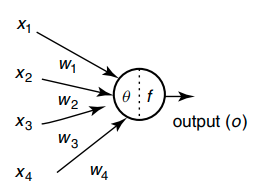
\includegraphics[width=0.5\textwidth]{imagenes/neuron}
        \end{center}
        \caption[Neurona Artificial]{}
    \end{figure}

Cada \textbf{neurona} realiza una operación simple: recibe varias entradas, las
pondera por medio de \textbf{pesos} $w_{i}$, suma estos valores junto con un \textbf{sesgo} $b$, y aplica una función
de activación.
La salida de la neurona se expresa como:

$z =w_{1}x_{1} + w_{2}x_{2} + \dots + w_{n}x_{n} + b_{z} = w_{1}x_{1} + w_{2}x_{2} + \dots + w_{n}x_{n} + b$

Luego, el valor $z$ pasa por una función de activación, que introduce la no linealidad en el sistema, permitiendo que
las redes neuronales modelen relaciones complejas.
    \item \textbf{Capas de la Red}:
    \begin{figure}[htp] \label{fig:capas-red-neuronal}
        \begin{center}
            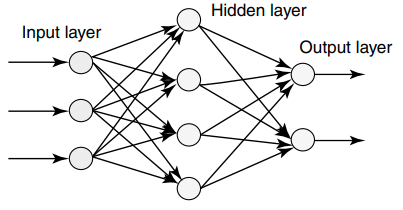
\includegraphics[width=0.5\textwidth]{imagenes/capas_red_neuronal}
        \end{center}
        \caption[Capas de la Red Neuonial Artificial]{}
    \end{figure}
\begin{itemize}
    \item \textbf{Capa de entrada}: Es la primera capa de la red neuronal, que recibe los datos crudos (por ejemplo,
píxeles de una imagen).
    \item \textbf{Capas ocultas}: Estas capas intermedias entre la entrada y la salida aprenden representaciones
abstractas de los datos.
En una red profunda, hay múltiples capas ocultas, lo que permite la \textbf{transformación jerárquica} de los datos.
    \item \textbf{Capa de salida}: Produce la predicción final, que puede ser una clase (en problemas de clasificación)
o un valor numérico (en problemas de regresión).
\end{itemize}
    \item \textbf{Pesos y Bias}: Los \textbf{pesos} son parámetros ajustables que determinan la importancia de cada
entrada en la neurona.
El \textbf{bias} es otro parámetro que se suma al valor ponderado para desplazar la activación de la neurona y permitir
que el modelo ajuste mejor los datos.

    \item \textbf{Funciones de Activación}: Las funciones de activación son fundamentales para que las redes neuronales
puedan aprender relaciones no lineales.
Entre las más comunes se encuentran:
\begin{itemize}
    \item \textbf{ReLU(Rectified Linear Unit)}: $ReLU(x)=\max(0,x)$, que activa solo valores positivos.
    \item \textbf{Sigmoide}: Que transforma los valores en un rango entre 0 y 1.
    \item \textbf{Tanh (Tangente hiperbólica)}: Transforma los valores en un rango entre -1 y 1.
\end{itemize}
\end{enumerate}

El uso de \textbf{backpropagation} o retropropagación permite ajustar los pesos y biases durante el entrenamiento
mediante un algoritmo de optimización, como el descenso de gradiente.
De esta manera, la red aprende minimizando la diferencia entre sus predicciones y las respuestas correctas.
\section{Redes Neuronales Convolucionales}\label{sec:redes-neuronales-convolucionales}
Las \textbf{Redes Neuronales Convolucionales} (Convolutional Neural Networks, CNNs) son una clase de redes neuronales
profundas especialmente efectivas para el procesamiento de datos que tienen una estructura de tipo rejilla, como las
imágenes.
Fueron inspiradas por el sistema visual de los mamíferos, donde diferentes capas de neuronas responden a estímulos
visuales de manera jerárquica. \\[2pt]

Las CNNs son ampliamente utilizadas en tareas de \textbf{visión por computador}, como el reconocimiento de imágenes, la
segmentación de objetos y la clasificación de imágenes.
Lo que diferencia a las CNNs de las redes neuronales tradicionales es su capacidad para detectar
\textbf{patrones espaciales} como bordes, texturas, y formas, sin necesidad de un procesamiento manual de las
características.


\subsection{Componentes principales de una CNN}\label{subsec:componentes-principales-de-una-cnn}
\begin{figure}[htp] \label{fig:convolution-layer}
    \begin{center}
        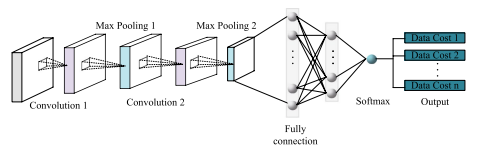
\includegraphics[width=1\textwidth]{imagenes/convolution_layer}
    \end{center}
    \caption[Puntos globales y locales]{En esta imagen extraída de
    \cite{A review of convolutional neural networks in computer vision} puede observarse de la estructura de una red
    neuronale convolucional. Junto a sus capas convolucionales. }
\end{figure}

\begin{enumerate}
    \item \textbf{Capas Convolucionales}: Estas capas aplican \textbf{filtros o kernels} sobre las imágenes de entrada
para detectar características locales, como bordes, esquinas o texturas.
Un filtro convolucional es una pequeña matriz que se mueve a lo largo de la imagen, calculando productos escalares en
cada posición para producir un mapa de características.

Las convoluciones son útiles porque explotan la \textbf{localidad de las características}, es decir, las relaciones
espaciales entre píxeles cercanos.
Además, la cantidad de parámetros se reduce drásticamente en comparación con las capas densas, ya que el filtro se
comparte a lo largo de la imagen.
    \item \textbf{Pooling (Submuestreo o Agrupamiento)}: Las capas de pooling reducen la dimensionalidad de las
características extraídas por las capas convolucionales, lo que hace que las representaciones sean más manejables y
robustas frente a pequeños cambios o desplazamientos en la imagen.

El max-pooling es la técnica de pooling más común, donde se toma el valor máximo dentro de una ventana de píxeles,
reduciendo el tamaño de la imagen, pero reteniendo las características más importantes.
    \item \textbf{Capas Densas}: Después de varias capas convolucionales y de pooling, se agregan una o más
\textbf{capas densas} (fully connected) para realizar la clasificación o predicción final.
Estas capas toman todas las características aprendidas en las capas convolucionales y las combinan para generar una
decisión final.
    \item \textbf{Batch Normalization}: Esta técnica se utiliza para \textbf{normalizar} las salidas de las capas
intermedias de una red neuronal.
Batch Normalization ayuda a \textbf{acelerar el entrenamiento} y a hacer que la red sea más estable, al reducir el
\textbf{desplazamiento covariante} (cambios en las distribuciones de las entradas de las capas intermedias a lo largo
del entrenamiento).
Esto se logra al normalizar las entradas de cada capa convolucional o densa antes de aplicar la activación, ajustando
su media y varianza.

    \item \textbf{Dropout}: El Dropout es una técnica de \textbf{regularización} que se utiliza para prevenir el
\textbf{sobreajuste} (overfitting) durante el entrenamiento de una red neuronal.
Durante cada iteración del entrenamiento, Dropout \textbf{desactiva aleatoriamente} un porcentaje de las neuronas, lo
que obliga a la red a no depender excesivamente de ciertas neuronas y a ser más robusta.
Esta técnica mejora la generalización de la red, lo que la hace funcionar mejor en datos no vistos.

\end{enumerate}

\subsection{Funcionamiento General de una CNN}\label{subsec:funcionamiento-general-de-una-cnn}
Al pasar una imagen a través de varias capas convolucionales, la red aprende a identificar características simples como
líneas y bordes.
Conforme avanza a capas más profundas, las características se vuelven más abstractas, capturando patrones más complejos
como formas, texturas y, finalmente, estructuras completas como objetos. \\[6pt]

Por ejemplo, en una red entrenada para reconocer caras, las primeras capas pueden detectar bordes o contornos, las
capas intermedias pueden aprender a reconocer ojos, nariz o boca, y las últimas capas pueden identificar una cara
completa.

\subsection{Aplicaciones de las CNN}\label{subsec:aplicaciones-de-las-cnn}
\begin{itemize}
    \item \textbf{Clasificación de imágenes}: Etiquetar imágenes en distintas categorías, como identificar animales o
vehículos.
    \item \textbf{Detección de objetos}: Identificar y localizar objetos en imágenes.
    \item \textbf{Reconocimiento facial}: Utilizado en sistemas de seguridad, como el desbloqueo de teléfonos móviles.
\end{itemize}

Las CNN son fundamentales en muchas aplicaciones modernas debido a su capacidad para procesar y entender datos visuales
de manera eficiente y automática.

\section{Datasets}\label{sec:datasets}
En el aprendizaje profundo, los datasets son colecciones de datos etiquetados o no etiquetados que se utilizan para
entrenar modelos.
Estos conjuntos de datos suelen contener ejemplos organizados que representan la entrada para el modelo, y en muchos
casos, también las etiquetas correspondientes que indican la salida deseada.
Los datasets varían en tamaño, calidad y tipo, dependiendo de la tarea a resolver, como la clasificación de imágenes,
el reconocimiento de patrones o la predicción de series temporales.

\subsection{Rock, Paper, Scissors (Piedra, Papel, Tijera)}\label{subsec:rock-paper-scissors}
\textbf{Rock, Paper, Scissors}~\cite{Rock Paper Scissors Dataset} fue creado originalmente por Laurence Moroney y se
utiliza para clasificar imágenes de las manos representando los gestos de `piedra', `papel' y `tijeras'.
El conjunto de datos contiene alrededor de 2,500 imágenes distribuidas en tres categorías: piedra, papel y tijeras.
Las imágenes están en color y tienen un tamaño de 300x300 píxeles. \\[6pt]

En este trabajo, se ha utilizado el dataset de \textbf{Rock, Paper, Scissors} para evaluar el rendimiento del modelo en
un problema de clasificación de imágenes más variado y natural, que involucra múltiples clases.
Además, permite explorar la eficacia de los algoritmos meméticos en un entorno más cercano al reconocimiento de
objetos, lo que añade mayor complejidad al problema.

\subsection{MNIST (Modified National Institute of Standards and Technology)}\label{subsec:mnist}
\textbf{MNIST}~\cite{MNIST Dataset} es uno de los datasets más utilizados en el campo del aprendizaje automático y el
aprendizaje profundo.
Contiene 70,000 imágenes de dígitos escritos a mano (60,000 para el conjunto de entrenamiento y 10,000 para el de
prueba).
Las imágenes son en escala de grises y tienen un tamaño de 28x28 píxeles, con cada píxel representando una intensidad
de color entre 0 (negro) y 255 (blanco).

Este dataset se utiliza comúnmente como \textbf{benchmark} para evaluar modelos de clasificación de imágenes,
particularmente en arquitecturas convolucionales.

La simplicidad de \textbf{MNIST} lo hace ideal para probar modelos de redes neuronales convolucionales, ya que ofrece un
equilibrio entre un problema fácil de entender, pero con suficiente complejidad para que los modelos más avanzados
demuestren mejoras.

\subsection{Comparación con otros datasets}\label{subsec:comparacion-con-otros-datasets}
La selección de estos dos datasets responde a la necesidad de evaluar los algoritmos meméticos en distintos niveles de
complejidad.
\textbf{MNIST}, con imágenes en escala de grises de bajo nivel de complejidad, proporciona una referencia clara y
estandarizada para comparar el rendimiento y la reducción de datos.
Por otro lado, el dataset de \textbf{Rock, Paper, Scissors} introduce más desafíos visuales y complejidades,
permitiendo analizar cómo los algoritmos meméticos se comportan en escenarios más complejos que podrían ser
representativos de aplicaciones más reales en visión por computadora.

\section{Modelos}\label{sec:modelos}
En el ámbito del aprendizaje profundo, existen diversas arquitecturas de redes neuronales convolucionales que han
demostrado un rendimiento excepcional en diversas tareas de visión por computadora.
Estas arquitecturas están diseñadas para abordar problemas complejos y variados, desde la clasificación de imágenes
hasta la detección de objetos y el segmentado de imágenes. \\[6pt]

A continuación, se explorarán algunas de estas arquitecturas que representan avances significativos en la eficiencia y
efectividad del aprendizaje profundo.

\subsection{ResNet50}\label{subsec:resnet50}
\textbf{ResNet50}~\cite{resnet} es una arquitectura de red neuronal convolucional introducida por Kaiming He et al. en 2015.
La principal innovación de ResNet es la introducción de \textbf{bloques de residualidad}, que permiten la construcción
de redes extremadamente profundas sin el problema de la degradación del rendimiento. \\[6pt]

La idea básica de los bloques residuales es permitir que la red aprenda funciones de identidad, facilitando así la
propagación de la información y el gradiente a través de la red.
En términos prácticos, esto se traduce en un rendimiento mejorado en tareas de clasificación de imágenes, donde
ResNet50 ha logrado resultados sobresalientes en competiciones como ImageNet. \\[6pt]

ResNet50 está compuesta por 50 capas, de las cuales 49 son capas convolucionales y una es una capa totalmente conectada.
La arquitectura incluye capas de normalización y activación (ReLU), así como una estructura que permite saltos de
conexión, lo que significa que la entrada de una capa se suma a la salida de una capa posterior.

\subsection{MobileNetV2}\label{subsec:mobilenet}
\textbf{MobileNet}~\cite{} es una arquitectura de red neuronal diseñada específicamente para aplicaciones móviles y de visión
por computadora en dispositivos con recursos limitados.
Introducida por Andrew G. Howard et al.\ en 2017, MobileNet se basa en el principio de
\textbf{convoluciones separables en profundidad} (depthwise separable convolutions), que dividen el proceso de
convolución en dos pasos: primero, se aplica una convolución a cada canal de la entrada (depthwise), y luego, se
combinan los resultados con una convolución 1x1 (pointwise). \\[6pt]

Esta técnica reduce significativamente el número de parámetros y el costo computacional, lo que permite ejecutar
modelos de visión por computadora en dispositivos móviles sin sacrificar drásticamente la precisión.

\subsubsection{MobileNetV2}\label{subsubsec:mobilenetv2}
\textbf{MobileNetV2}~\cite{}, introducido por Sandler et al.\ en 2018, mejora la arquitectura de MobileNet original al
incorporar varias innovaciones.
La principal contribución de MobileNetV2 es la introducción de los bloques de \textbf{residualidad invertida} (inverted
residuals), que permiten que la red mantenga una mayor capacidad de representación y flujo de información a través de
las capas. \\[6pt]

Además, MobileNetV2 utiliza una función de activación llamada \textbf{linear bottleneck}, que ayuda a preservar la
información durante la propagación a través de las capas, lo que mejora aún más el rendimiento del modelo en tareas de
clasificación y detección.
Esta arquitectura se optimiza para ser altamente eficiente, permitiendo que sea utilizada en aplicaciones de tiempo
real en dispositivos con limitaciones de hardware. \\[6pt]

MobileNetV2 ha demostrado ser una opción popular para aplicaciones en dispositivos móviles y sistemas embebidos,
ofreciendo un buen equilibrio entre precisión y eficiencia computacional.

\chapter{Repaso Bibliográfico}\label{ch:repaso_bibliografico}
%Repaso Bibliográfico: Revisión de trabajos previos relevantes en el área.
% !TeX root = ../proyecto.tex

\chapter{Descripción de los Algoritmos}\label{ch:descripcion-algoritmos}
En este capítulo se describen los diferentes algoritmos utilizados en el desarrollo de este trabajo.
Todos ellos tienen como objetivo principal reducir el tamaño del conjunto de datos de entrenamiento utilizado en los
modelos de aprendizaje profundo, con el fin de optimizar el rendimiento y reducir el costo computacional.
El enfoque adoptado en este trabajo es la aplicación de algoritmos meméticos, los cuales combinan principios de
algoritmos genéticos con estrategias de búsqueda local.


A continuación, se detallan los algoritmos principales implementados en este proyecto: el \textbf{algoritmo aleatorio},
el \textbf{algoritmo de búsqueda local} y el \textbf{algoritmo genético}

\section{Algoritmo Aleatorio}\label{sec:algoritmo-aleatorio}
%Algoritmos Meméticos: Detalla qué son y cómo se aplican a la reducción de datos.
El \textbf{algoritmo aleatorio} sirve como referencia básica para medir la efectividad de los algoritmos más avanzados.
Este enfoque selecciona subconjuntos de datos de manera completamente aleatoria, sin aplicar ningún tipo de estrategia
de optimización.

\subsection{Descripción}\label{subsec:descripcion}
El algoritmo comienza tomando el conjunto de datos completo y seleccionando una fracción de los ejemplos de
entrenamiento de forma aleatoria.
Esta selección se realiza sin ningún criterio basado en la relevancia de los datos, lo que implica que el conjunto de
entrenamiento resultante puede no ser representativo o puede contener redundancias innecesarias.

\subsection{Aplicación en la reducción de datos}\label{subsec:aplicacion-en-la-reduccion-de-datos}
A pesar de su simplicidad, el \textbf{algoritmo aleatorio} puede ser útil como método de comparación.
En muchos casos, los algoritmos más complejos deben demostrar que pueden superar este enfoque básico en términos de
precisión y eficiencia.
Al seleccionar datos de manera aleatoria, este método a menudo produce conjuntos de entrenamiento subóptimos, lo que
resulta en modelos menos precisos o con mayor varianza.

\subsection{Resultados esperados}\label{subsec:resultados-esperados}
Debido a la naturaleza aleatoria del algoritmo, los resultados son altamente variables.
Es probable que en muchas ejecuciones el rendimiento del modelo entrenado sea inferior al obtenido con métodos más
estructurados.
Este algoritmo proporciona una línea base importante para evaluar la efectividad de los algoritmos más avanzados.


\section{Algoritmo Búsqueda Local}\label{sec:algoritmo-busqueda-local}
El \textbf{algoritmo de búsqueda local} es una técnica más sofisticada que explora el espacio de soluciones de manera
más estructurada, buscando mejorar progresivamente una solución inicial.

\subsection{Descripción}\label{subsec:descripcion2}
La búsqueda local se basa en la idea de comenzar con una solución inicial (un subconjunto de datos) y realizar pequeños
cambios o `movimientos' en esa solución para explorar otras soluciones cercanas.
En este contexto, cada solución es un subconjunto de datos.
El algoritmo evalúa diferentes subconjuntos de datos probando si estos mejoran el rendimiento del modelo de aprendizaje
profundo al entrenarlo con ellos.


El proceso básico de la búsqueda local es el siguiente:
\begin{enumerate}
      \item Se genera una solución inicial, por ejemplo, seleccionando un subconjunto de datos aleatoriamente.
      \item Se realizan cambios locales en la solución, como añadir o eliminar ejemplos del conjunto de datos.
      \item Se evalúa la nueva solución según el rendimiento del modelo de aprendizaje profundo.
      \item Si la nueva solución es mejor, se reemplaza la solución actual por esta.
      \item El proceso se repite hasta que no se observan mejoras significativas o hasta que se alcanza un número
      \item predefinido de iteraciones.
\end{enumerate}

\subsection{Aplicación en la reducción de datos}\label{subsec:aplicacion-en-la-reduccion-de-datos2}
En el contexto de la reducción de datos, el objetivo de la búsqueda local es identificar un subconjunto más pequeño de
ejemplos que sea suficiente para entrenar el modelo con un rendimiento similar al obtenido con el conjunto de datos
completo.
La búsqueda local explora el espacio de posibles subconjuntos, eliminando ejemplos redundantes o irrelevantes, y
conservando solo aquellos que son cruciales para el rendimiento del modelo.

\subsection{Ventajas y limitaciones}\label{subsec:ventajas-y-limitaciones}
\textbf{Ventajas}: Este enfoque permite una exploración más exhaustiva del espacio de soluciones que un algoritmo
aleatorio.
Al hacer pequeños ajustes en cada iteración, el algoritmo puede encontrar mejores soluciones de manera eficiente.
\textbf{Limitaciones}: Sin embargo, la búsqueda local puede quedarse atrapada en \textbf{óptimos locales}, es decir,
soluciones que parecen buenas en comparación con las cercanas, pero que no son globalmente óptimas.

\section{Algoritmos Genéticos}\label{sec:algoritmos-geneticos}
Los \textbf{algoritmos genéticos} son algoritmos de búsqueda inspirados en los principios de la evolución natural.
En este trabajo, se aplican con el objetivo de encontrar subconjuntos óptimos de datos de entrenamiento, reduciendo el
tamaño del conjunto mientras se mantiene o mejora el rendimiento del modelo de aprendizaje profundo.

\subsection{Descripción}\label{subsec:descripcion3}
El funcionamiento de los algoritmos genéticos se basa en los conceptos de \textbf{selección natural},
\textbf{cruzamiento} y \textbf{mutación}.
El proceso se puede resumir en los siguientes pasos:
\begin{enumerate}
      \item \textbf{Inicialización}: Se genera una población inicial de posibles soluciones, cada una de ellas
            representando un subconjunto del conjunto de datos.
      \item \textbf{Evaluación}: Cada subconjunto de datos (o `individuo') es evaluado entrenando el modelo con ese
            subconjunto y midiendo su rendimiento.
      \item \textbf{Selección}: Se seleccionan los mejores individuos de la población basándose en su rendimiento.
            Los mejores individuos tienen más probabilidades de ser seleccionados para la siguiente generación.
      \item \textbf{Cruzamiento}: Se combinan pares de individuos seleccionados para crear nuevos subconjuntos.
            Esto se realiza intercambiando ejemplos entre los subconjuntos.
      \item \textbf{Mutación}: Con una pequeña probabilidad, se realizan cambios aleatorios en algunos individuos, como
            añadir o eliminar ejemplos del subconjunto.
      \item \textbf{Iteración}: El proceso de evaluación, selección, cruzamiento y mutación se repite durante varias
            generaciones, con la esperanza de que cada generación produzca soluciones mejores que la anterior.
\end{enumerate}

\subsection{Aplicación en la reducción de datos}\label{subsec:aplicacion-en-la-reduccion-de-datos3}
Los \textbf{algoritmos genéticos} son especialmente adecuados para la reducción de datos porque permiten explorar un
espacio de soluciones muy amplio de manera eficiente.
La combinación de individuos y la introducción de mutaciones aleatorias permiten al algoritmo escapar de los óptimos
locales, un problema común en la búsqueda local.

El uso de algoritmos genéticos para reducir datos en este contexto implica encontrar subconjuntos de entrenamiento que
proporcionen un buen equilibrio entre tamaño y rendimiento.
Esto se logra al evaluar diferentes subconjuntos y mejorar las soluciones generación tras generación.

\subsection{Ventajas y limitaciones}\label{subsec:ventajas-y-limitaciones2}
\textbf{Ventajas}: Los algoritmos genéticos son efectivos para explorar grandes espacios de soluciones y tienen una
gran capacidad para evitar quedar atrapados en óptimos locales.
Son especialmente útiles en problemas donde la solución óptima no es evidente desde el principio.


\textbf{Limitaciones}: Estos algoritmos pueden ser costosos computacionalmente, ya que requieren evaluar muchas
soluciones a lo largo de múltiples generaciones.
Además, su convergencia a veces puede ser lenta, dependiendo del tamaño del espacio de búsqueda y de los
parámetros del algoritmo (tamaño de la población, tasa de mutación, etc.).

\subsection{Versiones}\label{subsec:versiones}

% !TeX root = ../proyecto.tex

\chapter{Implementación}\label{ch:implementacion}
En este capítulo se presenta en detalle la arquitectura técnica del sistema implementado, incluyendo los componentes y
módulos principales, las herramientas específicas empleadas en la construcción del sistema, y los elementos clave para
optimizar el rendimiento de los algoritmos y su evaluación.


\section{Descripción del Sistema}\label{sec:descripcion-del-sistema}
%Descripción del Sistema: Detalla la arquitectura del sistema que estás implementando.
La estructura del proyecto se organizó modularmente para facilitar el acceso, el mantenimiento y la extensibilidad del código fuente.
La organización de carpetas es la siguiente:
\begin{itemize}
      \item \texttt{data} -- Conjunto de datos utilizados en los experimentos.
      \item \texttt{docs} -- Documentación del proyecto en latex.
            \begin{itemize}
                  \item \texttt{bibliografia} -- Archivos relacionados con las referencias bibliográficas.
                  \item \texttt{capitulos} -- Archivos individuales para cada capítulo del documento.
                  \item \texttt{config} -- Archivos de configuraciones de la documentación LaTeX.
                  \item \texttt{imagenes} -- Imágenes utilizadas en la documentación.
                  \item \texttt{out} -- Archivos generados por el compilador de LaTeX.
                  \item \texttt{portada} -- Archivo portada del documento.
                  \item \texttt{prefacio} -- Archivo prefacio del documento.
                  \item \texttt{proyecto.tex} -- Archivo principal de LaTeX que compila el documento.
            \end{itemize}
      \item \texttt{img} -- Imágenes generadas automáticamente durante los experimentos.
      \item \texttt{LICENSE} -- Términos de distribución del proyecto.
      \item \texttt{logs} -- Registros de las ejecuciones, incluyendo tiempos de inicio, fin y resultados intermedios de los algoritmos.
      \item \texttt{README.md} -- Descripción general.
      \item \texttt{requirements.txt} -- Dependencias del proyecto.
      \item \texttt{results} -- Resultados de los experimentos.
            \begin{itemize}
                  \item \texttt{csvs} -- Resultados de las ejecuciones guardados en tablas.
                  \item \texttt{salidas} -- Salidas en bruto de consola.
            \end{itemize}
      \item \texttt{scripts} -- Scripts de ejecución automática, comparación de experimentos y generación de gráficos finales.
      \item \texttt{src} -- Código fuente principal del proyecto.
            \begin{itemize}
                  \item \texttt{algorithms} -- Implementaciones de los algoritmos.
                  \item \texttt{main.py} -- Módulo principal de ejecución individual.
            \end{itemize}
      \item \texttt{tmp} -- Ficheros temporales generados durante la ejecución.
      \item \texttt{utils} -- Módulos de apoyo, como clases auxiliares, generación de gráficos y funciones utilitarias.
\end{itemize}

El código completo del proyecto, incluyendo los scripts, algoritmos, documentación y resultados,
se encuentra disponible en el repositorio público de GitHub: \url{https://github.com/JoseRuizLopez/TFG}.


\section{Herramientas y Lenguajes de Programación}\label{sec:herramientas-y-lenguajes-de-programacion}
%Herramientas y Lenguajes de Programación: Lista las herramientas y tecnologías que usarás.
El desarrollo del proyecto se ha llevado a cabo utilizando \textbf{Python 3.10}~\cite{vanderplasPythonDataScience2016} como
lenguaje principal, debido a su versatilidad y amplia adopción en el campo del \textbf{aprendizaje profundo} y la
\textbf{manipulación de datos}.
Python es conocido por su facilidad de uso, extensibilidad y la gran cantidad de bibliotecas disponibles para el
procesamiento de datos y la implementación de modelos de \textbf{machine learning}.


Las principales bibliotecas empleadas durante el desarrollo son las siguientes:
\begin{itemize}
      \item \textbf{PyTorch 2.3.1}~\cite{ketkarIntroductionPyTorch2021, TorchcudaPyTorch24}: Para la construcción,
            entrenamiento y optimización de modelos de aprendizaje profundo.
            PyTorch fue elegido por su flexibilidad y capacidad para ejecutarse eficientemente en GPU\@.
      \item \textbf{Scikit-learn 1.5.2}~\cite{vanderplasPythonDataScience2016}: Para la evaluación de los modelos se utilizaron
            métricas estándar~\cite{kramerScikitLearn2016}.
            Su API permite una integración fluida con PyTorch y otros módulos.
      \item \textbf{Numpy 2.0.0}~\cite{NumPyV20Manual}: Para operaciones matemáticas y manipulación de matrices,
            siendo una herramienta esencial en el procesamiento de datos.
      \item \textbf{Polars 1.9.0}~\cite{PolarsPythonAPI}: Biblioteca para manejar DataFrames de gran tamaño,
            elegida por su rendimiento superior en comparación con Pandas.
      \item \textbf{Matplotlib 3.9.2}~\cite{Matplotlib393Documentation}: Biblioteca utilizada para la generación y
            visualización de gráficas.
      \item \textbf{Seaborn 0.13.2}~\cite{Seaborn0132Documentation}: Estilización avanzada de gráficos estadísticos.
      \item \textbf{Openpyxl 3.1.5}~\cite{Openpyxl313Documentation}: Generación automática de archivos Excel a partir de resultados experimentales.
\end{itemize}

Cada una de estas herramientas fue seleccionada por su robustez y su idoneidad para cumplir con los requisitos
específicos del proyecto, facilitando tanto la implementación de los algoritmos meméticos como la reducción y el
análisis de los datos utilizados en los modelos de aprendizaje profundo.

\section{Gestión de Dependencias}\label{sec:gestion-de-dependencias}
Para garantizar que el proyecto se ejecute correctamente y todas las bibliotecas necesarias estén disponibles, se ha
utilizado un archivo \texttt{requirements.txt}.
Este archivo contiene una lista de todas las bibliotecas y sus versiones específicas que el proyecto requiere.


Para el \textbf{desarrollo local}, se ha optado por crear un entorno virtual utilizando
\texttt{venv}~\cite{CreationVirtualEnvironments}.
Esta práctica permite aislar las dependencias del proyecto de otros proyectos en la máquina, evitando conflictos entre
versiones de bibliotecas.


Para la \textbf{implementación en el servidor}, se ha utilizado \texttt{conda}~\cite{CondaDocumentation} como gestor
de paquetes y entornos.
Conda facilita la gestión de entornos y la instalación de bibliotecas, especialmente en configuraciones más complejas.



Esto facilita la reproducibilidad del proyecto y minimiza posibles conflictos de versión, lo que es fundamental para
mantener la integridad del código y el rendimiento de las aplicaciones.

\section{Arquitectura de la Implementación}\label{sec:arquitectura-de-la-implementacion}
La arquitectura de la implementación desarrollada para este trabajo está diseñada con un enfoque modular y escalable,
que permite gestionar de forma eficiente las distintas fases del proceso de selección de instancias y evaluación de modelos.
El sistema se compone de varios módulos interrelacionados que se encargan de la generación de subconjuntos,
la ejecución de los algoritmos evolutivos y meméticos, la evaluación de las soluciones mediante modelos preentrenados, y la visualización y almacenamiento de resultados.
Esta estructura facilita la incorporación de nuevos algoritmos o mejoras en los ya existentes, garantizando una mayor flexibilidad y mantenimiento del código.

\subsection{Esquema General de Funcionamiento de los Algoritmos}\label{subsec:esquema-algoritmos}
El funcionamiento general de los algoritmos implementados en este trabajo sigue un flujo estructurado y modular que permite una ejecución ordenada de todas las etapas del proceso.
La Figura~\ref{fig:esquema-flujo-algoritmos} muestra el esquema general de funcionamiento, desde la configuración inicial hasta la evaluación final de resultados.

\begin{figure}[htp]
      \centering
      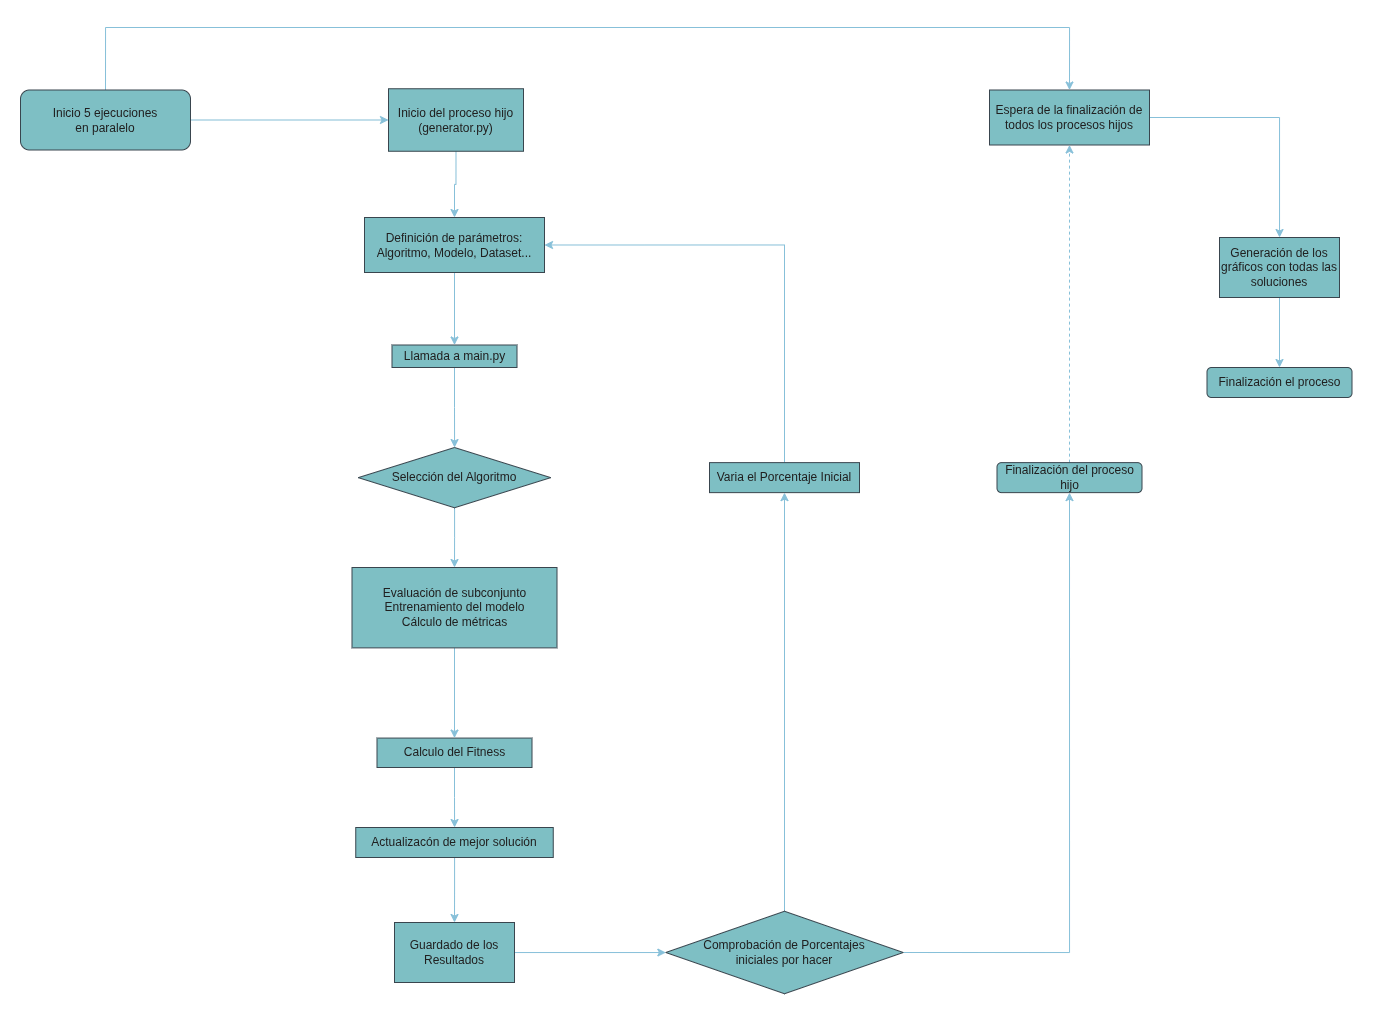
\includegraphics[width=0.95\textwidth]{imagenes/flujo2.drawio}
      \caption{Esquema general del flujo de ejecución de los algoritmos y evaluación de subconjuntos.}
      \label{fig:esquema-flujo-algoritmos}
\end{figure}

El proceso se organiza en los siguientes pasos principales:

\begin{enumerate}
      \item \textbf{Ejecución del script de paralelización:} Se inicia el script que permite ejecutar múltiples experimentos de manera paralela,
            facilitando la obteción de resultados de diferentes semillas.
      \item \textbf{Configuración inicial:} Se define el algoritmo, el modelo y el dataset a utilizar, a través de los parámetros en \texttt{generator.py}.
      \item \textbf{Ejecución del núcleo principal:} El script \texttt{main.py} se encarga de orquestar la ejecución,
            llamando a las funciones específicas según el algoritmo seleccionado.
      \item \textbf{Generación y evaluación de subconjuntos:} Cada algoritmo genera subconjuntos de datos de entrenamiento a partir del conjunto original.
      \item \textbf{Entrenamiento del modelo:} Se realiza el entrenamiento del modelo utilizando los subconjuntos generados,
            aplicando técnicas de \textit{transfer learning} con modelos preentrenados.
      \item \textbf{Almacenamiento de resultados:} Cada evaluación almacena los resultados obtenidos (métricas y composición del subconjunto) y,
            tras finalizar la ejecución, se generan gráficos como boxplots y visualizaciones que permiten analizar el rendimiento de cada enfoque.
\end{enumerate}

\subsection{Configuración de Modelos Preentrenados}\label{subsec:configuracion-modelos-preentrenados}
En este trabajo, se han utilizado modelos convolucionales preentrenados como base para la tarea de clasificación de imágenes.
Concretamente, se han empleado las arquitecturas \textbf{ResNet50} y \textbf{MobileNetV2},
cargadas con pesos preentrenados sobre \texttt{ImageNet} o \texttt{CIFAR10}, según el dataset utilizado en cada experimento.

Para adaptar estos modelos a la tarea específica de clasificación de subconjuntos de datos,
se ha seguido una estrategia de \textit{transfer learning} que permite reducir significativamente el coste computacional del entrenamiento.
Esta estrategia consiste en congelar todas las capas del modelo, excepto la última,
de manera que las representaciones aprendidas en la etapa preentrenada puedan ser reutilizadas como extractores de características generales.

Específicamente, la \textbf{última capa} de cada modelo preentrenado (la capa densa o \textit{fully connected})
ha sido reemplazada por una nueva capa completamente conectada (\texttt{Linear}) adaptada al número de clases del dataset en uso.
Esta capa es la única que se entrena durante la fase de evaluación de cada subconjunto generado por los algoritmos,
permitiendo obtener métricas como \textit{accuracy}, \textit{precision}, \textit{recall} y \textit{F1-score} de forma eficiente.

El uso de pesos preentrenados y la congelación de capas proporcionan varias ventajas:
\begin{itemize}
      \item Reducción del tiempo de entrenamiento en cada evaluación.
      \item Aprovechamiento de representaciones genéricas previamente aprendidas, lo que mejora la generalización.
      \item Adaptabilidad de los modelos a distintos datasets y tareas, modificando únicamente la capa final.
\end{itemize}

Este enfoque se implementa mediante las herramientas de PyTorch,
congelando explícitamente los gradientes de todas las capas del modelo y definiendo la nueva capa final con el número adecuado de salidas para cada problema de clasificación.

\subsection{Módulo de Algoritmos}\label{subsec:modulo-de-algoritmos}
Ubicado en \texttt{src/algorithms/} este módulo contiene las implementaciones principales de los
algoritmos desarrollados en el proyecto.

Este módulo utiliza la arquitectura GPU para maximizar la velocidad de ejecución y está diseñado para ser escalable,
permitiendo la inclusión de nuevos operadores meméticos si es necesario.

\subsection{Núcleo de Ejecución}\label{subsec:nucleo-de-ejecucion}
El módulo \texttt{main.py} centraliza la ejecución de un experimento individual, inicializando configuraciones,
entrenando el modelo y generando gráficos.

Los pasos de la función principal de \texttt{main.py} es:
\begin{enumerate}
      \item \textbf{Establece Configuración Inicial}: Configura una semilla, elige el dataset y prepara un archivo de log.
      \item \textbf{Inicia el Proceso del Algoritmo}: Según el nombre del algoritmo (algoritmo) especificado, se llama a
            la función correspondiente (por ejemplo, genetic\_algorithm, memetic\_algorithm, etc.).
      \item \textbf{Almacena Resultados}: Una vez que el algoritmo termina, registra la duración, los resultados y la
            métrica final en un archivo.
      \item \textbf{Visualiza Resultados}: Si hay datos de fitness, genera una gráfica de la evolución del fitness a lo
            largo del proceso.
      \item \textbf{Genera un Resumen}: Calcula estadísticas adicionales (como porcentaje de clases seleccionadas en
            Paper, Rock y Scissors), y devuelve estos resultados junto con el historial de fitness.
\end{enumerate}

\subsection{Módulo de Utilidades}\label{subsec:modulo-de-utilidades}
La carpeta \texttt{utils/} contiene funciones auxiliares:
\begin{itemize}
      \item \textbf{utils\_plot.py}: Generación de gráficos.
      \item \textbf{classes.py}: Definición de enumeraciones para algoritmos, métricas, datasets y modelos.
      \item \textbf{utils.py}: Funciones de ayuda como el cálculo de métricas o la creación de diccionarios de selección de imágenes.
\end{itemize}

Estos módulos se encargan de generar gráficas comparativas entre distintos porcentajes o algoritmos y en
generar un CSV con los datos finales para ser analizados.

\subsection{Scripts de Ejecución en GPU}\label{subsec:scripts-de-ejecucion-en-gpu}
En scripts, se encuentran los programas necesarios para ejecutar los algoritmos en un servidor GPU, lo que permite
maximizar la eficiencia en el entrenamiento y la evaluación de modelos.
\begin{enumerate}
      \item \textbf{Configuración de GPU}: Los scripts están configurados para identificar y utilizar las GPU disponibles
            en el servidor, reduciendo los tiempos de entrenamiento de modelos.
      \item \textbf{Optimización de Ejecución}: Se implementaron configuraciones de batch size y técnicas de
            procesamiento paralelo en PyTorch, aprovechando la memoria y el poder de procesamiento de las GPU\@.
\end{enumerate}

Estos scripts están diseñados para ser ejecutados en un entorno de servidor, reduciendo los tiempos de prueba en el
entorno local y permitiendo un análisis iterativo más rápido.

\section{Consideraciones de Optimización}\label{sec:consideraciones-de-optimizacion}
Durante el desarrollo, se optimizaron varios aspectos para mejorar el rendimiento del sistema:

\begin{enumerate}
      \item \textbf{Aceleración en GPU}: Todas las operaciones de cálculo intensivo fueron migradas a la GPU mediante
            PyTorch.
      \item \textbf{Uso Eficiente de Memoria}: Con Polars y Numpy, se optimizó el manejo de grandes volúmenes de datos,
            utilizando tipos de datos específicos para reducir el uso de memoria.
      \item \textbf{Automatización de Evaluaciones}: Las pruebas de rendimiento se automatizaron, permitiendo una
            evaluación continua sin intervención manual.
      \item \textbf{Control de reproducibilidad}: Se fijaron semillas aleatorias en todas las librerías involucradas
            (random, numpy, torch, cuda) y se desactivaron los algoritmos no deterministas de cuDNN~\cite{CuBLASDeterministicAlgorithms}.
            Esta medida garantiza que las ejecuciones del sistema produzcan resultados consistentes entre sesiones,
            algo esencial en entornos de evaluación comparativa.
      \item \textbf{Diagnóstico automático de GPU}: Implementación de un script (cuda-diagnostic.py) que comprueba disponibilidad
            de CUDA y dispositivos antes de lanzar experimentos, garantizando un entorno correcto.
\end{enumerate}

Además, se implementó un mecanismo de \textbf{early stopping} basado en la ausencia de mejora del valor de fitness durante
un número determinado de evaluaciones consecutivas.
Aunque no se utiliza una pérdida de validación explícita como en enfoques tradicionales, este enfoque funcionalmente cumple el mismo propósito:
detener el algoritmo cuando se detecta estancamiento, reduciendo así el coste computacional innecesario~\cite{EarlyStoppingDiscussion2024}.


Gracias a estas optimizaciones, el sistema permite explorar un amplio abanico de configuraciones de manera eficiente, manteniendo la robustez y estabilidad de los resultados.

\section{Métricas de Evaluación}\label{sec:metricas-evaluacion}

Para evaluar el rendimiento de los modelos de clasificación utilizados en los experimentos,
se han empleado cuatro métricas estándar en el ámbito del aprendizaje automático: \textbf{accuracy}, \textbf{precisión}, \textbf{recall} y \textbf{F1-score}.
Dado que se trata de un problema multiclase, estas métricas se han calculado utilizando el promedio \textit{macro},
lo que implica computarlas individualmente para cada clase y luego obtener la media aritmética.

A continuación se describen y formalizan cada una de estas métricas:

\begin{itemize}
      \item \textbf{Accuracy} (exactitud): representa la proporción de predicciones correctas sobre el total de ejemplos.
            $$
                  Accuracy = \frac{TP + TN}{TP + TN + FP + FN}
            $$
            En el caso multiclase, se generaliza como:
            $$
                  \mathrm{Accuracy} = \frac{\text{Número de predicciones correctas}}{\text{Total de predicciones}}
            $$

      \item \textbf{Precisión}: mide cuántas de las instancias clasificadas como positivas fueron realmente positivas.
            En el caso multiclase (macro), se calcula como:
            $$
                  \text{Precisión}_{\text{macro}} = \frac{1}{C} \sum_{i=1}^{C} \frac{TP_i}{TP_i + FP_i}
            $$

      \item \textbf{Recall}: indica cuántas de las instancias realmente positivas fueron correctamente identificadas por el modelo:
            $$
                  \mathrm{Recall}_{\text{macro}} = \frac{1}{C} \sum_{i=1}^{C} \frac{TP_i}{TP_i + FN_i}
            $$

      \item \textbf{F1-score}: es la media armónica entre precisión y recall, útil cuando se desea un equilibrio entre ambas:
            $$
                  \mathrm{F1\text{-}score}_{\text{macro}} = \frac{1}{C} \sum_{i=1}^{C} \frac{2 \cdot \text{Precisión}_i \cdot \text{Recall}_i}{\text{Precisión}_i + \text{Recall}_i}
            $$
\end{itemize}

Donde:
\begin{itemize}
      \item $TP_i$: verdaderos positivos de la clase $i$
      \item $FP_i$: falsos positivos de la clase $i$
      \item $FN_i$: falsos negativos de la clase $i$
      \item $C$: número total de clases
\end{itemize}

Para facilitar la comprensión de estos conceptos, en la Figura~\ref{fig:matriz-confusion} se muestra una representación gráfica de una matriz de confusión.
\begin{figure}[H]
      \centering
      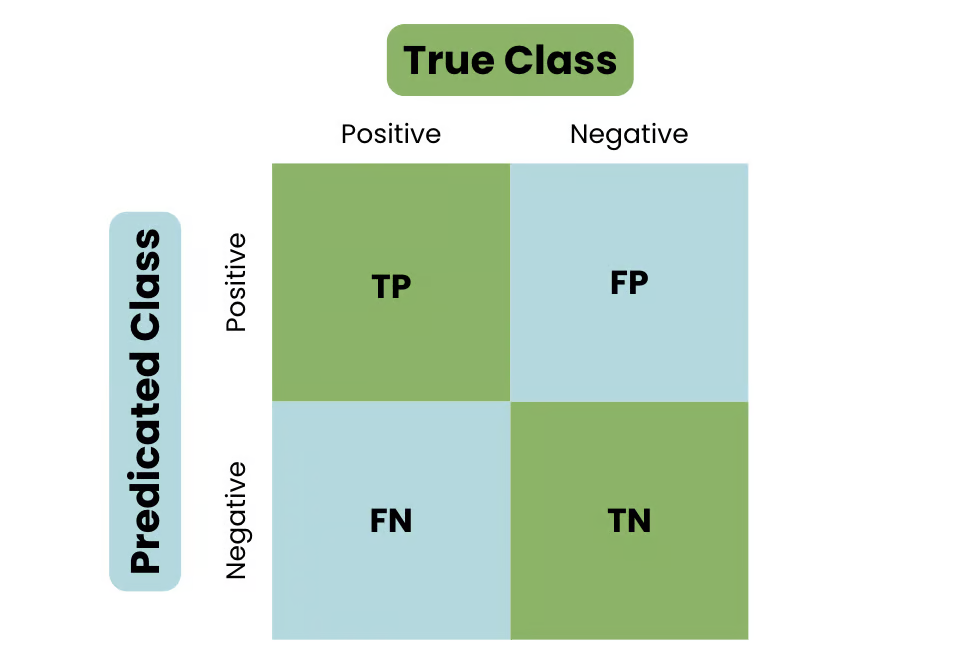
\includegraphics[width=0.5\textwidth]{imagenes/matriz-de-confusion.png}
      \caption{Representación gráfica de una matriz de confusión}
      \label{fig:matriz-confusion}
\end{figure}

Estas métricas fueron implementadas utilizando la librería \texttt{scikit-learn}, que permite su cálculo eficiente a partir de las
predicciones del modelo y las etiquetas reales del conjunto de validación.

\chapter{Desarrollo Experimental}\label{ch:desarrollo_experimental}

Las pruebas iniciales que se plantearon fueron tomar un dataset simple para realizar las primeras pruedas, y ya cuando
funcionase correctamente, probar con otro dataset más complejo o realista.
Para ello se decidió usar el dataset de \textbf{RPS}~\cite{}, ya que tiene un número pequeño de imagenes, 2520 en el
\textbf{training set} y 3 clases (840 imágenes por clase), y 372 imagenes para el \textbf{test set} (124 por clase).
\\[6pt]

Para obtener unos primeros resultados con este dataset, se planteó usar el modelo de \textbf{Resnet50}~\cite{}.
Se hicieron unas pruebas con distintos porcentajes para ver cuál era el porcentaje que más merecia la pena usar.
\\[6pt]

Tras realizar las pruebas iniciales, se pensó en probar con otro modelo, uno más veloz para que tardase menos tiempo en
realizar pruebas y poder realizar más pruebas en menos tiempo.
Para ello se decido usar \textbf{Mobilenet}~\cite{}, debido a que es más rápido y suele tener resultados parecidos si
los Dataset no son muy grandes ~\cite{ResnetVsMobilenet}.

% !TeX root = ../proyecto.tex

\chapter{Conclusiones}\label{ch:conclusiones}

% Bibliografía y apéndices
\chapter{Bibliografía}\label{ch:bibliografia}
\printbibliography[heading=none, category=cited]


%\appendix
%\input{apendices/manual_usuario/manual_usuario}
%\input{glosario/entradas_glosario}

\chapter*{}
\thispagestyle{empty}

\end{document}
% !TEX root = proyecto.tex
